\subsubsection{UCS 1 - Autenticazione al Server}
\begin{figure}[h]
    \centering
    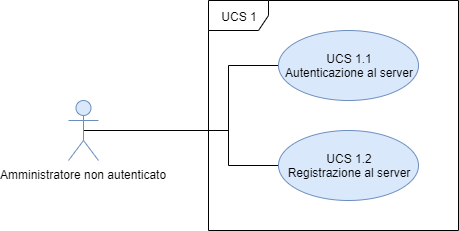
\includegraphics[scale=0.6]{sezioni/UseCase/Immagini/UCS1.png}
    \caption{Autenticazione\ap{G} al Server}
\end{figure}

\begin{itemize}
\item \textbf{Attori primari:} Amministratore non autenticato\ap{G};
\item \textbf{Precondizione:} L'amministratore non è autenticato\ap{G};
\item \textbf{Postcondizione:} L'amministratore è stato autenticato\ap{G} e può avere accesso alle funzionalità offerte dal sistema;
\item \textbf{Scenario principale:} Amministratore non identificato inserisce il nome utente e la password per autenticarsi al server;
\item \textbf{Flusso di eventi:}
    \begin{enumerate}
        \item UCS 1.1 - Inserimento e-mail;
        \item UCS 1.2 - Inserimento password;
        \item UCS 1.3 - Password dimenticata;
    \end{enumerate}
\item \textbf{Estensioni:}
	\begin{enumerate}		
		\item UCS 1.4 - Credenziali errate.
	\end{enumerate}
\end{itemize}

\subsubsection{UCS 1.1 - Inserimento e-mail}%sea level
\begin{itemize}
\item \textbf{Attori primari:} Utente non autenticato\ap{G};
%\item \textbf{Attori secondari:}%opzionale
\item \textbf{Precondizione:} L'amministratore non è autenticato\ap{G};
\item \textbf{Postcondizione:} L'amministratore ha inserito il proprio e-mail.
\end{itemize}

\subsubsection{UCS 1.2 - Inserimento password}%sea level
\begin{itemize}
\item \textbf{Attori primari:} Amministratore non autenticato\ap{G};
%\item \textbf{Attori secondari:}%opzionale
\item \textbf{Precondizione:} L'amministratore non è autenticato\ap{G};
\item \textbf{Postcondizione:} L'amministratore ha inserito la propria password.
\end{itemize}

\subsubsection{UCS 1.3 - Password dimenticata}%sea level
\begin{itemize}
\item \textbf{Attori primari:} Amministratore non autenticato\ap{G};
%\item \textbf{Attori secondari:}%opzionale
\item \textbf{Precondizione:}  L'amministratore non autenticato\ap{G} clicca su cambio password;
\item \textbf{Postcondizione:} L'amministratore ha cambiato password;
\item \textbf{Scenario principale:} L'amministratore non autenticato\ap{G} ha intenzione di modificare la propria password;
\item \textbf{Flusso di eventi:}
    \begin{enumerate}
        \item UCS 1.3.1 - Inserimento e-mail;
        \item UCS 1.3.2 - E-mail cambio password;
        \item UCS 1.3.3 - Nuova password;
        \item UCS 1.3.4 - Conferma nuova password;
        \item UCS 1.3.5 - Pulsante cambio password.
    \end{enumerate}
\end{itemize}

\subsubsection{UCS 1.3.1 - Inserimento e-mail}
\begin{itemize}
\item \textbf{Attori primari:} Amministratore non autenticato\ap{G};
\item \textbf{Precondizione:} L'amministratore non è autenticato\ap{G}; %è nella schermata di password dimenticata
\item \textbf{Postcondizione:} L'amministratore ha inserito l'e-mail.
\end{itemize}

\subsubsection{UCS 1.3.2 - E-mail cambio password}
\begin{itemize}
\item \textbf{Attori primari:} Amministratore non autenticato\ap{G};
\item \textbf{Precondizione:} L'amministratore non è autenticato\ap{G};
\item \textbf{Postcondizione:} L'amministratore riceve l'email per il cambio password [UCS 1.3.3 - UCS 1.3.4].
\end{itemize}

\subsubsection{UCS 1.3.3 - Nuova password}
\begin{itemize}
\item \textbf{Attori primari:} Amministratore non autenticato\ap{G};
\item \textbf{Precondizione:}  L'amministratore non è autenticato\ap{G};
\item \textbf{Postcondizione:} L'amministratore inserisce la nuova password.
\end{itemize}

\subsubsection{UCS 1.3.4 - Conferma nuova password}
\begin{itemize}
\item \textbf{Attori primari:} Amministratore non autenticato\ap{G};
\item \textbf{Precondizione:} L'amministratore non è autenticato\ap{G};
\item \textbf{Postcondizione:} L'amministratore reinserisce la nuova password per confermarla.
\end{itemize}

\subsubsection{UCS 1.3.5 - Pulsante cambio password}%fish level
\begin{itemize}
\item \textbf{Attori primari:} Amministratore non autenticato\ap{G};
\item \textbf{Precondizione:} L'amministratore non è autenticato\ap{G};
\item \textbf{Postcondizione:} L'amministratore ha selezionato di cambio password.
\end{itemize}

\subsubsection{UCS 1.4 - Credenziali errate}%sea level
\begin{itemize}
\item \textbf{Attori primari:} Amministratore non autenticato\ap{G};
%\item \textbf{Attori secondari:}%opzionale
\item \textbf{Precondizione:} L'amministratore non è autenticato\ap{G};
\item \textbf{Postcondizione:} L'amministratore ha la possibilità di reinserire le sue credenziali o di cambiarle [UCS 1.1 e UCS 1.2].
\end{itemize}

\subsubsection{UCS 1.5 - Pulsante accedi}%sea level
\begin{itemize}
\item \textbf{Attori primari:} Amministratore non autenticato\ap{G};
%\item \textbf{Attori secondari:}%opzionale
\item \textbf{Precondizione:} L'amministratore non è autenticato\ap{G};
\item \textbf{Postcondizione:} L'amministratore ha selezionato il pulsante d'accesso al server.
\end{itemize}
